\section{Experiments}

\subsection{Z-score Versus Activation-score}

Z-score is one of the most used methods in linguistic statistics. It compares the observed frequency of a word with the frequency expected in case of a "normal" distribution. This calcul gives easily for example the most specific vocabulary of a given author in a contrastive corpora. The highest z-score are the most specific word in this case. This is a simple but strong method to analyze feature on text. It can be also used to classify word sequences according to the global z-score (sum of the score) in the sequence. The mean accuracy of this methods on our data set is around 85\%, that confirm z-score is really meaningful on contrastive data. On the other hand, the deep learning reaches most of time more than 90\% on text classification. It means the training methods can learn also by themselves some sort of linguistic specificities useful to distinguish class of text or authors. We've seen on image that's the role of the convolution. It learns an abstraction on the data to make classification easier. The question is : what is the nature of this abstraction on text ? We going to seen now that the deep learning detect automatically words with hight z-score but apparently it's not this only linguistic marks detected.

\begin{figure}[h]
\begin{center}
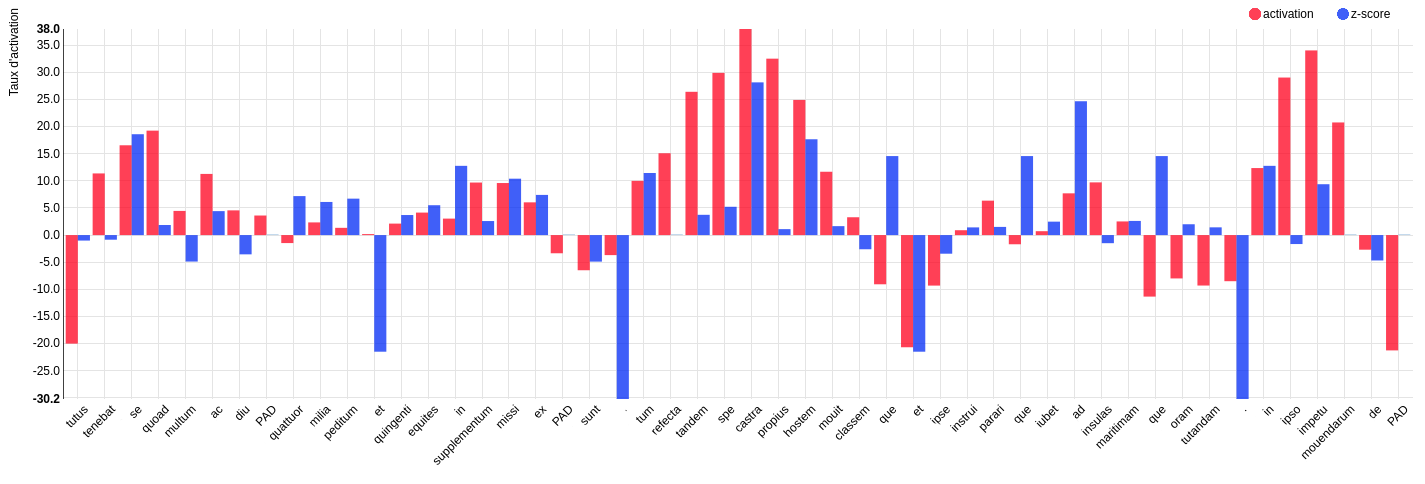
\includegraphics[width=16cm]{img/z-score_activations.png}
\caption{Latin dataset : Livius Book XXIII Chap. 26 - Z-score Vs Activation-score}
\label{comparision}
\end{center}
\end{figure}

The Figure \ref{comparision} shows us a comparison between z-score and activation-score on a sequence extract form our latin corpora. Here it's an example where Livius\footnote{Lucius Livius Andronicus (c. 284 – c. 205 BC) was a Greco-Roman dramatist and epic poet of the Old Latin period} use some specific words. As we can see, when the z-score is the highest the activation-score around is also very high (word \textit{castra}). But not always, for example small words as \textit{que}, \textit{ad} and \textit{et} are also high in z-score but they not activate the network as the same level. We saw in (reference ****) that deeplearning is more sensible with long words, but we can see also on Figure \ref{comparision} that word like \textit{tenebat}, \textit{multum} or \textit{propius} are totally uncorrelated. If we make the Pearson\footnote{Pearson correlation coefficient measures the linear relationship between two datasets. It has a value between $+1$ and $-1$, where $1$ is total positive linear correlation, $0$ is no linear correlation, and $-1$ is total negative} correlation coefficient on this sequence, we obtain 0.38. Not a hight correlation so, and this example one of the most correlated example of our dataset.

\subsection{Dataset : English}


\subsection{Dataset : French}

" …notre pays advienne, à l'école pour nos enfants, au travail pour l'ensemble de nos concitoyens, pour le climat, pour le quotidien de chacune et chacun d' entre vous. Ces transformations profondes ont commencé et se poursuivront avec la même force, le même rythme, la même intensité"

Cet extrait issu du discours de vœux d'Emmanuel Macron (31 décembre 2017) est mal attribué par l'ADT (Z-score) qui le rapproche statistiquement de De Gaulle, et bien attribué par le Deep learning qui reconnait du Macron.
L'erreur d'attribution statistique s'explique par une phraséologie très gaullienne et la multiplication de marqueurs linguistiques fortement indicés chez de Gaulle : par exemple, de Gaulle avait pour caractéristique de faire des phrases longues et littéraires articulées autour de conjonctions de coordination  comme " et " (z-score = 28 chez de Gaulle, 2 occurrences dans l'extrait). Son discours était également plus conceptuel que la moyenne, et cela se traduisait par une sur-utilisation des articles définis (le, la, l', les) très nombreux dans  l'extrait (7 occurrences) ; particulièrement au féminin singulier (" la " République, " la " liberté, " la " nation ", " la " guerre, etc ; ici " la " même force, " la " même intensité).

Les meilleures performances du deep learning interrogent quant à elle le linguiste et épouse parfaitement ce que l'on sait socio-linguistiquement du discours dynamique de Macron.
La zone d'activation la plus importante de l'extrait concerne le syntagme nominal " transformation profonde ".
Pris séparément, aucun des deux mots du syntagme n'est très macronien d'un point de vue statistique (" transformation " = XXX ; " profonde " = YYY). Mieux : le syntagme lui-même n'est pas attesté dans le corpus d'apprentissage du Président (0 occurrence). 
Cependant, on peut constater que la co-occurrence de " transformation " et de " profonde " s'élève à +XXX chez Macron : ce n'est donc pas l'occurrence d'un mot seul, ou de l'autre, qui est macronienne mais l'apparition simultanée des deux dans une même fenêtre.
Pour autant, la cooccurrence de " transformation " et de " profonde " ne saurait être suffisante pour caractériser Macron, notamment parce que la cooccurrence des deux mots est plus fréquente encore chez Pompidou par exemple ; d'autres indices additionnés sont nécessaires à l'attribution.
Les zones d'activation secondes et complémentaires de l'extrait concernent ainsi les deux verbes " advienne " et " poursuivront ".
D'un point de vue sémantique, les deux verbes conspirent parfaitement, après le syntagme  " transformation profonde ", à donner la dynamique nécessaire à un discours qui prône le changement. Mais c'est les temps verbaux (portés par la morphologie des verbes) qui apparaissent déterminants dans l'analyse.
Le calcul des codes grammaticaux co-occurrents au mot " transformation " indique ainsi que les verbes au subjonctif et les verbes au futur (et également les noms) sont les codes privilégies chez Macron. (GRAPH XXX)
Plus précisément encore, l'algorithme indique que, chez Macron, lorsque " transformation " est associée à un verbe au subjonctif (ici "advienne "), alors il existe le plus souvent un verbe au futur co-présent (ici " poursuivront ").
" Transformation profonde ", " advenir " au subjonctif, " poursuivre " au futur : tous ces éléments signent, ensemble, un discours fait de promesse d'action, dans la bouche d'un président jeune et dynamique.
Enfin, le graphique indique que " transformation " est surtout associée aux noms chez le Président : dans une concentration extraordinaire, l'extrait en recense ainsi 11 ( " pays ", " école ", " enfants ", " travail ", " concitoyens ", " climat ", " quotidien ", " transformations ", " force ", " rythme ", " intensité ").


\subsection{Dataset : Latin}

